% \documentclass[journal,draftclsnofoot,onecolumn]{IEEEtran}
\documentclass[conference, draftclsnofoot, letterpaper]{IEEETran}
\usepackage{listings}
\usepackage[utf8]{inputenc}
\usepackage{xcolor}   
\usepackage{enumitem}     
\usepackage{float}
\usepackage{graphicx}
\usepackage{tcolorbox}
\usepackage{url}

\begin{document}

\title{CSC3050 Computer Architecture \\Project 1 Report}

\author{\IEEEauthorblockN{Chenhao~Wu~(117010285)}
\IEEEauthorblockA{The Chinese University of Hong Kong, Shenzhen.}
}


\maketitle


\section{Introduction}

In this assignment, we are required to implement an assembler that interprets MIPS assembly files into their corresponding binary executable, as well as a simulator that accepts the executable and simulates the execution of MIPS instructions. This article is the final report of this assignment, aiming to show how we designed and implemented the assembler and simulator. The instruction encoding and decoding formats are all specified by the official documentation and textbook. Also, the register file and memory bar are simulated according to the manual and TA's instructions. All the coding work in this project is implemented with C/C++ and we have verified the functional correctness of assembling and simulation results on a Linux virtual machine. In this report, we also aim to illustrate the implementation details of each sub-module in our submitted work. 

We organize this report into three sections. In the first section, we will introduce the execution data flow of the submitted assembler and simulator, including the arguments, options, and format of input/output files involved in each individual step. In the second section, we will briefly introduce the implementation details of the submitted assembler and simulator, e.g. how the basic function is implemented, for instance like how the program encodes MIPS assembly line into binary codes. In the last section, we will show the testing results of assembler/simulator from test cases given by the teaching team. 


\section{Execution Data Flow} 

\subsubsection{Kick-Start Executable}

To simplify the testing flow for people who do not familiar with the implementation details but wish to test our implementation with minimal efforts, we include an executable in the cmakelists which will be built by default. 

\begin{tcolorbox}
	\$ mkdir build \&\& cd build \&\& cmake .. \&\& make 
\end{tcolorbox}

The content of this executable is shown as follows: 

\definecolor{listinggray}{gray}{0.9}
\definecolor{lbcolor}{rgb}{0.9,0.9,0.9}
\lstset{
	backgroundcolor=\color{lbcolor},
	tabsize=4,    
	%   rulecolor=,
	language=[GNU]C++,
	basicstyle=\scriptsize,
	upquote=true,
	aboveskip={1\baselineskip},
	columns=fixed,
	showstringspaces=false,
	extendedchars=false,
	breaklines=true,
	prebreak = \raisebox{0ex}[0ex][0ex]{\ensuremath{\hookleftarrow}},
	frame=single,
	numbers=left,
	showtabs=false,
	showspaces=false,
	showstringspaces=false,
	identifierstyle=\ttfamily,
	keywordstyle=\color[rgb]{0,0,1},
	commentstyle=\color[rgb]{0.026,0.112,0.095},
	stringstyle=\color[rgb]{0.627,0.126,0.941},
	numberstyle=\color[rgb]{0.205, 0.142, 0.73},
	%        \lstdefinestyle{C++}{language=C++,style=numbers}’.
}
\lstset{
	backgroundcolor=\color{lbcolor},
	tabsize=4,
	language=C++,
	captionpos=b,
	tabsize=3,
	frame=lines,
	numbers=left,
	numberstyle=\tiny,
	numbersep=5pt,
	breaklines=true,
	showstringspaces=false,
	basicstyle=\scriptsize,
	%  identifierstyle=\color{magenta},
	keywordstyle=\color[rgb]{0,0,1},
	commentstyle=\color{Darkgreen},
	stringstyle=\color{red}
}


\begin{lstlisting}
#include "psim.hh"

int main(int argc, char** argv) {
	Simulator simulator;
	simulator_init(&simulator, argc, argv);
	simulator_exec(&simulator);
	simulator_free(&simulator);
}
\end{lstlisting}

In general, this executable will initialize a simulator instance and accept given command line options. According to the user arguments, the program will proceed the subsequent flow of assembler and simulator. In specific, our simulator accepts following command line options: 

\begin{figure*}
	\centering
	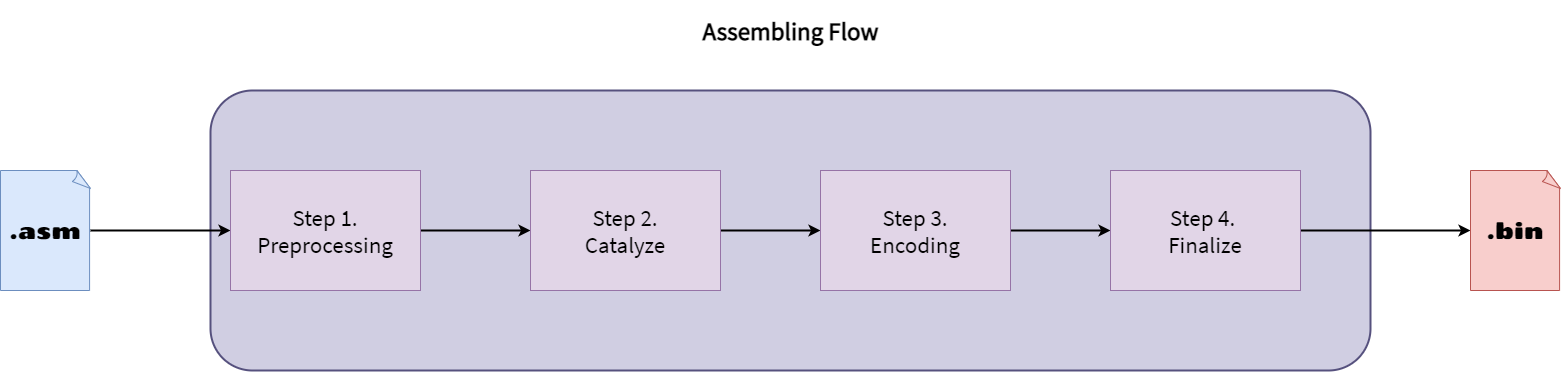
\includegraphics[width=.9\linewidth]{asm_flow}
	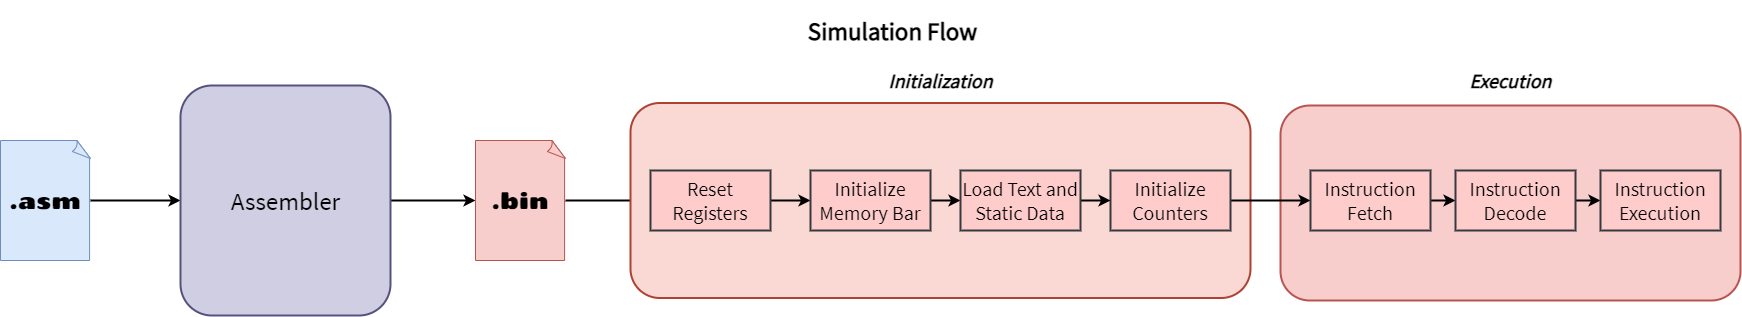
\includegraphics[width=\linewidth]{sim_flow}
	\caption{The upper-side figure shows each step of the assembling flow and the bottom-side figure shows each step of the simulation flow}
	\label{fig::flow}
\end{figure*}

\begin{tcolorbox}
	\footnotesize
\begin{itemize}\itemsep .5em
	\item \textit{\textbf{--verbose}}: specify this option to enable a detailed and informative logging during the program execution. 
	\item \textit{\textbf{--ELF [ELF\_FILE]}}: the ELF file argument specifies the path to assembly file.
	\item \textit{\textbf{--input\_file [INPUT\_FILE]}}: the input file argument specifies the path to a file which prestores the \emph{user inputs} in the simulation. 
	\item \textit{\textbf{--full\_flow}}: specify this option to enable both assembling and simulation in a run (if this option is NOT specified, the program will omit the simulation and only run the assembling routines).
	\item \textit{\textbf{--output\_bin [OUTPUT\_FILE]}}: the path to the output binary executable of the program. 
	\item \textit{\textbf{--output\_stdout [OUTPUT\_FILE]}}: the path to the standard output file of the program. 
	\item \textit{\textbf{--help}}: show help message.
\end{itemize}
\end{tcolorbox}


Follows are several examples to launch the program:
	
\begin{enumerate}[label=(\roman*)]\itemsep .5em
	\footnotesize
	\item \textbf{Assemble \emph{testfiles/ttassembler/1.in} to its binary:}
	
	\textit{\color{red}./psim --ELF testfiles/ttassembler/1.in --output\_bin 1.out}
	
	\item \textbf{Assemble and simulate \emph{a-plus-b.asm}}
	
	\textit{\color{red}./psim --ELF a-plus-b.asm --input\_file}
	\textit{\color{red}a-plus-b.in --output\_stdout a-plus-b.out}
		\item \textbf{Assemble and simulate \emph{a-plus-b.asm} (and show the result in stdout)}
		
		\textit{\color{red}./psim --ELF a-plus-b.asm --input\_file a-plus-b.in}
	\end{enumerate}
Above commands could be frequently used in the testing. Also, in the last section we will show the corresponding results of these command as well. 

\subsubsection{Assembling flow}

In general, the assembler accepts an assembly file as input, and produces a binary file as output. Specifically, the process is being handled in four steps:

\begin{enumerate}[label=(\roman*)]\itemsep .5em
	\item \textit{\textbf{Preprocessing: }} In this step, the assembler will read an assembly file line by line and perform several preprocessing on the original assembly file. First, the assembler will remove comments (starting with a sharp sign) and blank lines from the file. Secondly, the assembler will detect \emph{.text} and \emph{.data} labels and separate the original assembly file into text section and data section. 
	
	\item \textit{\textbf{Catalyze:}} In this step, the assembler will catalyze the content of the text and data section for further encoding and simulation. Because MIPS instructions do not encode a label in binary, all the labels have to be substituted by addresses or corresponding offsets before the encoding begins. Thus, the assembler will first collect all the prescribed labels in the text section with a written form: \emph{label:} and then store the mapping between labels and the corresponding address of the instruction it refers to. Then, the assembler will substitute all the labels in the text section with either absolute addresses (for jumping instructions) or offsets (for branching instructions). 
	
	In addition, if command line argument \emph{--full\_flow} is specified, the assembler will parse the data string in \emph{.data} section and store all the static data in memory bar during this step. Need to mention that, our assembler can only support 5 types of data type in \emph{.data} section, i.e. \emph{.ascii}, \emph{.asciiz}, \emph{.half}, \emph{.byte}, \emph{.word}.
	
	\item \textit{\textbf{Encoding:}} In this step, the assembler proceeds to encode all the instructions into their binary form with respect to the encoding format specified in the official documentation and textbook. Since the number of required instructions is limited, we hardcoded all the encoding formats in our code.
	
	\item \textit{\textbf{Finalize:}} In this step, the assembler will free some resources and variables that will no longer be used in the subsequent steps. If command-line argument \emph{--output\_bin} is passed, in the finalizing step assembler will store the encoded binary executable in the assigned output file.
\end{enumerate}

The overall execution flow of assembler is shown in the upper-side figure of Fig \ref{fig::flow}.

\subsubsection{Simulation flow}

If command line option \emph{--full\_flow} is specified, the program will proceed to perform simulation on the assembled binary executable. The simulation consists of 7 steps:

\begin{itemize}
	\item \textbf{Initialization}
	\begin{enumerate}[label=(\roman*)]\itemsep .5em
		\item The simulator resets the value of all 34 registers (32 integer register, \emph{HI}, and \emph{LO} register) into zero.
		\item The simulator initializes a memory bar with required size space and reset the related counters/pointers such as \emph{\$sp}, \emph{MEM\_TEXT\_END}, \emph{MEM\_DYNAMIC\_END}, etc.
		\item The simulator loads text and static data into the text and static area of the memory bar. Need to notice that, if the simulation starts from assembling, the static data will be loaded during the catalyze step in instead. 
		\item The simulator initializes counters related to execution, e.g. \emph{program counter}.
	\end{enumerate}
	\item \textbf{Execution}
	\begin{enumerate}[label=(\roman*)\itemsep .5em]
		\setcounter{enumi}{4}
		\item The simulator fetches instructions (4-byte word) from address specified by the \emph{program counter}. The simulator will terminates execution and exits once the \emph{program counter} reaches the end of text section. 
		\item The simulator decodes the fetched instruction and routes to the corresponding routine.
		\item The simulator executes the instruction routine and increment the \emph{program counter} by 4 when execution finished.
	\end{enumerate}
\end{itemize}

The overall execution flow of simulator is shown in the bottom-side figure of Fig \ref{fig::flow}.

\section{Implementation Details}

\subsection{Assembler}

In our implementation, the assembler instance is defined by a \textit{structure type} with several data elements that closely relates to the assembling process. The defined structure type and contained data fields are shown as follows: 
\begin{lstlisting}
struct Assembler {
	std::string ELF_path;
	std::vector<std::string> content;
	std::vector<std::string> text_section;
	std::vector<uint32_t> bin;
	std::map<std::string, uint32_t> label_map;
	Options *user_options;
	MMBar *mmBar;
};
\end{lstlisting}

Specifically, \emph{ELF\_path} will be initialized with the filename of the input assembly, and the content of input assembly will be loaded to \emph{content} variable. After catalyze, mapping between labels and instruction addresses will be stored in \emph{label\_map}, and the text lines will be stored in the \emph{text\_section}. After assembling finished, the binary lines will be stored in the \emph{bin} variable. Along with these variables, pointer of user options (\emph{user\_options}) are passed to control the assembling flow and pointer of memory bar (\emph{mmBar}) are passed to store the static data in the memory bar.  

\begin{lstlisting}
void assembler_init(Assembler *assembler, std::string ELF_path, bool loadFromELF);
void assembler_exec(Assembler *assembler);
void assembler_free(Assembler *assembler);
\end{lstlisting}

In general, assembling processes can be called by above three functions, \emph{assembler\_init()}, \emph{assembler\_exec()}, and \emph{assembler\_free()}.

\subsection{Simulator}

Similar to assembler, the simulator instance is defined by a structure type as well. The defined structure type and contained data fields are shown as follow:

\begin{lstlisting}
struct Simulator {
	Assembler assembler;
	MMBar mmBar;
	Options user_options;
	std::vector<std::string> inputs;
	uint32_t current_input;
	std::vector<uint32_t> bin;
	uint32_t pc;
};
\end{lstlisting}
As shown in section 2.1, users could call three functions to launch the simulation, i.e. \emph{simulator\_init()}, \emph{simulator\_exec()}, and \emph{simulator\_exit()}. 

\subsubsection{Registers}

In our program we use an constant-length array to represent the register file hold by the simulator, shown as follows

\begin{lstlisting}
#define REG_NUM 34
	
extern int32_t register_file[REG_NUM];
extern double f_register_file[2];

int32_t register_file[REG_NUM] = {0};
double f_register_file[2] = {0};
\end{lstlisting}

\subsubsection{Memory Bar}

To simulate a memory bar in the interconnect system, we defined a MMBar structure as follows:
\begin{lstlisting}
#define MEM_SIZE 0x80000000UL
#define MEM_TEXT_START 0x400000UL
#define MEM_TEXT_END 0x500000UL
#define MEM_STACK_START 0xA00000UL
#define MEM_TOP MEM_STACK_START
#define MEM_DATA_START MEM_TEXT_END
struct MMBar {
	uint8_t *_memory;
	uint32_t text_end_addr;
	uint32_t static_end_addr;
	uint32_t dynamic_end_addr;
	bool initialized = false;
};
\end{lstlisting}
as well as following functions to manage and access the memory bar:
\begin{lstlisting}
	void mmbar_init(MMBar *mmBar);
	void mmbar_load_text(MMBar *mmBar, std::vector<std::uint32_t> bin);
	void mmbar_free(MMBar *mmBar);
	bool mmbar_write(MMBar *mmBar, uint32_t addr, uint8_t e);
	bool mmbar_writeu16(MMBar *mmBar, uint32_t addr, uint16_t e);
	bool mmbar_writeu32(MMBar *mmBar, uint32_t addr, uint32_t e);
	uint8_t mmbar_read(MMBar *mmBar, uint32_t addr);
	uint16_t mmbar_readu16(MMBar *mmBar, uint32_t addr);
	uint32_t mmbar_readu32(MMBar *mmBar, uint32_t addr);
	uint32_t mmbar_allocate(MMBar* mmBar, uint32_t size_n);
	void mmbar_load_static_u8(MMBar* mmBar, uint8_t e);
\end{lstlisting}

To guarantee the data integrity, all the subroutines should access (i.e. read/write) the memory element by calling \textit{mmbar\_*()} functions instead of directly accessing the internal array \textit{\_memory}.

\subsubsection{Execution}


Among all the subroutines, the most important subroutine is a loop that keep fetching instructions and increment the program counter by 4, shown as follows. This loop essentially triggers the finite-state machine and pushes the simulation into the next stage until its termination.  \footnote{Due to the page limit, we could not dive into each subroutine and describe them in detail, but we will keep updating the documentations in \url{https://github.com/Vito-Swift/Parch} to help folks understand the implementation of this simulator.}

\begin{lstlisting}
	void __simulator_exec_run(Simulator *simulator) {
		while (simulator->pc != simulator->mmBar.text_end_addr) {
			uint32_t b = mmbar_readu32(&simulator->mmBar, simulator->pc);
			if (!decode(simulator, b)) 
				exit(1);	
			simulator->pc += 4;
		}
	}
\end{lstlisting}

\subsection{Testing by gtest}

In the project we also include several google test executable which was originally designed for verifying the functional correctness of our assembler and simulator. However, since google test libraries are not installed in most testing environments, these tests will not be built by default. 

\section{Testing Results}

In this section we show 1 assembler tests and 3 simulator tests, with corresponding invoked commands and simulation results. The testing environment is specified as follows:

\begin{itemize}
	\item \textbf{Operating System: } Ubuntu@Linux 4.40
	\item \textbf{GNU C++ Compiler Version:} 7.5.0
	\item \textbf{CMake Version:} 3.17.3
	\item \textbf{CPU:} Intel Xeon E5-2699 v4@2.20GHz
	\item \textbf{Memory: } 315 GBytes
\end{itemize}

\subsection{Assembler Tests}

\begin{lstlisting}[language={}]
$ ./simulator --ELF ../PSim/test/testfiles/ttassembler/2.in --output_bin 2.out
$ cat 2.out
00100000100001001111111111111111
\end{lstlisting}

\subsection{Simulation Tests}

\subsubsection{a-plus-b.asm}

~\
\begin{lstlisting}[language={}]
$ ./simulator --ELF ../PSim/test/testfiles/ttsimulator/a-plus-b.asm --input_file ../PSim/test/testfiles/ttsimulator/a-plus-b.in --output_stdout a-plus-b.out --full_flow
$ cat a-plus-b.out
628
\end{lstlisting}

\subsubsection{fib.asm}

~\
\begin{lstlisting}[language={}]
$ ./simulator --ELF ../PSim/test/testfiles/ttsimulator/fib.asm --input_file ../PSim/test/testfiles/ttsimulator/fib.in --output_stdout fib.out --full_flow
$ cat fib.out
fib(16) = 987
\end{lstlisting}

\subsubsection{memcpy-hello-world.asm}

~\
\begin{lstlisting}[language={}]
$ ./simulator --ELF ../PSim/test/testfiles/ttsimulator/memcpy-hello-world.asm --input_file ../PSim/test/testfiles/ttsimulator/memcpy-hello-world.in --full_flow
hello, world
\end{lstlisting}

\end{document}